\begin{figure}
\centering
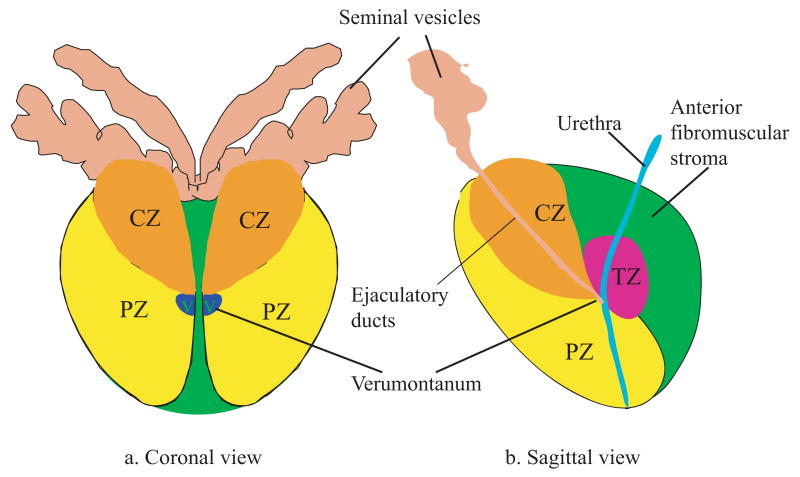
\includegraphics[width=0.75\linewidth]{figs/Mcneal_Zonal_Anatomy.jpg}
\caption{\textbf{Diagrams of McNeal’s zonal anatomy of the human
    prostate.~\cite{mcneal_path} It divides a human prostate into one
    non-glandular zone (the anterior fibromuscular stroma) and three glandular
    zones: central zone, peripheral zone and transition zone, denoted by CZ, PZ
    and TZ, respectively. (a) Coronal section of the prostate. V represents the
    verumontanum. (b) Sagittal section of the prostate. In the top part of the
    diagram, the seminar vesicles and ductus deferens enter the central zone
    and connect to the ejaculatory ducts, which merge with the urethra at the
    verumontanum. (Figure reprinted with permission.~\cite{Zhai2010a})}}
\label{fig:mcneal_anatomy} 
\end{figure}
